\documentclass[hyperref=colorlinks]{beamer}
\mode<presentation>
\usetheme{iclpt}
\setbeamertemplate{navigation symbols}{}
\setbeamertemplate{headline}{
\begin{beamercolorbox}[leftskip=.2cm,rightskip=.2cm,topskip=.2cm,ht=1.1cm,dp=0.1cm,wd=\textwidth]{institute in head/foot}
  
\includegraphics[height=1cm]{icl.pdf}
  \hfill
  
\includegraphics[height=1cm]{../Pics/CMS-Color.pdf}
\end{beamercolorbox}
}
\setbeamertemplate{footline}{
\begin{beamercolorbox}[ht=.55cm,dp=0.4cm,wd=\textwidth,leftskip=.3cm]{author in head/foot}%
  \begin{minipage}[c]{5cm}%
    \usebeamerfont{author in head/foot}
    \insertshortauthor 
    \insertshorttitle
    \end{minipage}\hfill%
  \insertframenumber{} / \pageref{lastframe}
  \hfill
  \begin{minipage}{6cm}
    \hfill
  \end{minipage}
\end{beamercolorbox}%
}

\usepackage{color}
\usepackage{tabularx,colortbl}
\usepackage{graphicx}
\usepackage{pdfpages}
\usepackage{feynmp}
\DeclareGraphicsRule{*}{mps}{*}{}

\title{\vspace{-0.2cm} Trigger Efficiency Measurements in Re-Reco Data}
%\subtitle{Paper - HIG-13-030, PASs: HIG-13-013, HIG-13-018, HIG-13-028 \vspace{-0.7cm}}
\author[P. Dunne]{\underline{P. Dunne} }%\\ on behalf of the H$\rightarrow$invisible analysis groups} % A.M. Magnan and A. Nikitenko Joao Pela with \\ R. Aggleton, J. Brooke: Bristol \\ C.Asawangtrakuldee, Q.Li: Peking \\ P. Srimanobhas: Chulalongkorn \\ S. Kumar, K. Mazumdar: Mumbai}
\titlegraphic{
  \vspace{-0.7cm}
  %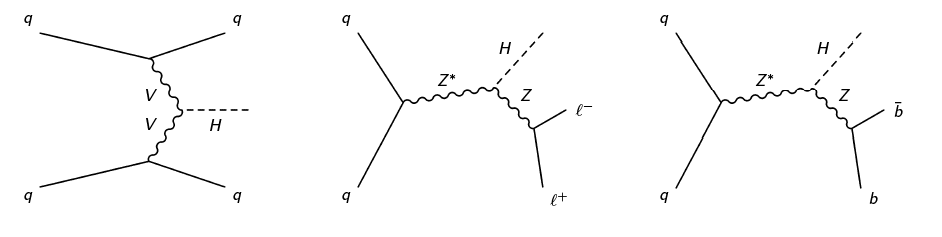
\includegraphics[width=\textwidth]{TalkPics/invcomb021213/feyndiags}
%% \begin{fmfgraph*}(100,70)
%%         \fmfleft{i1,i2}
%%         \fmfright{o1,o2,o3}
%%         \fmf{fermion}{i1,v1,o1}
%%         \fmf{fermion}{i2,v2,o3}
%%         \fmf{phantom,tension=4/5}{v1,v2}
%%         \fmffreeze
%%         \fmf{photon,label=$W,,Z$}{v1,v3}
%%         \fmf{photon,label=$W,,Z$}{v2,v3}
%%         \fmf{dashes}{v3,o2}
%%         \fmflabel{$q$}{i1}
%%         \fmflabel{$q$}{i2}
%%         \fmflabel{$q$}{o1}
%%         \fmflabel{$q$}{o3}
%%         \fmflabel{$H$}{o2}
%%       \end{fmfgraph*}
}
\date{}
\begin{document}
\begin{fmffile}{hig1330approvalfeynmandiags}

%TITLE PAGE
\section{Title}
\begin{frame}
  \titlepage
  
\end{frame}

%OUTLINE
\begin{frame}
  \frametitle{Overview}
  \begin{block}{}
    \scriptsize
  \begin{itemize}
  \item Last time I presented 1D efficiencies for met, mjj and jet 2 pt
  \item The following changes were made:
  \item[-] Check the difference between the cuts used and those used by Phat for the paper
  \item[-] Get the $\Delta\eta_{jj}$ turn on
  \item[-] Check the effect of applying the L1 Trigger
  \item Preliminary results from 3D efficiency studies have been produced

    \end{itemize}
  \end{block}
\end{frame}

 \begin{frame}
  \begin{block}{}
    \centering
    \begin{tabular}{|l|c|c|}
      \hline
      Variable & My Cut & Phat's Cut \\
      \hline
      $M_{jj}$ & $>$ 1100 & $>$1000 \\
      met & pfMet$>$130 & metnomuon$>$200 \\
      $jet 1 pt$ & $>$50 & $>$55 \\
      $jet 2 pt$ & $>$50 & $>$55 \\
      $\Delta\eta_{jj}$ & $>$4.2 & $>$4.2 \\
      $\Delta\phi_{jj}$ & No cut & No cut \\
      $\eta_{j1}\cdot\eta_{j2}$ & $<$0 & $<$0 \\
      CJV & No cut & Cut \\
      L1 met & No cut & $>$40 \\
      \hline
    \end{tabular}
  \end{block}
  \begin{block}{}
    \begin{itemize}
    \item Main differences are in L1 and Reco met cuts
    \item Minor differences in jet pt cuts and CJV
    \end{itemize}
  \end{block}
\end{frame}

\begin{frame}
  \frametitle{MET}
  \scriptsize
  \begin{columns}
    \column{.55\textwidth}
    \begin{block}{\scriptsize L1 met $>$ 40 GeV}
      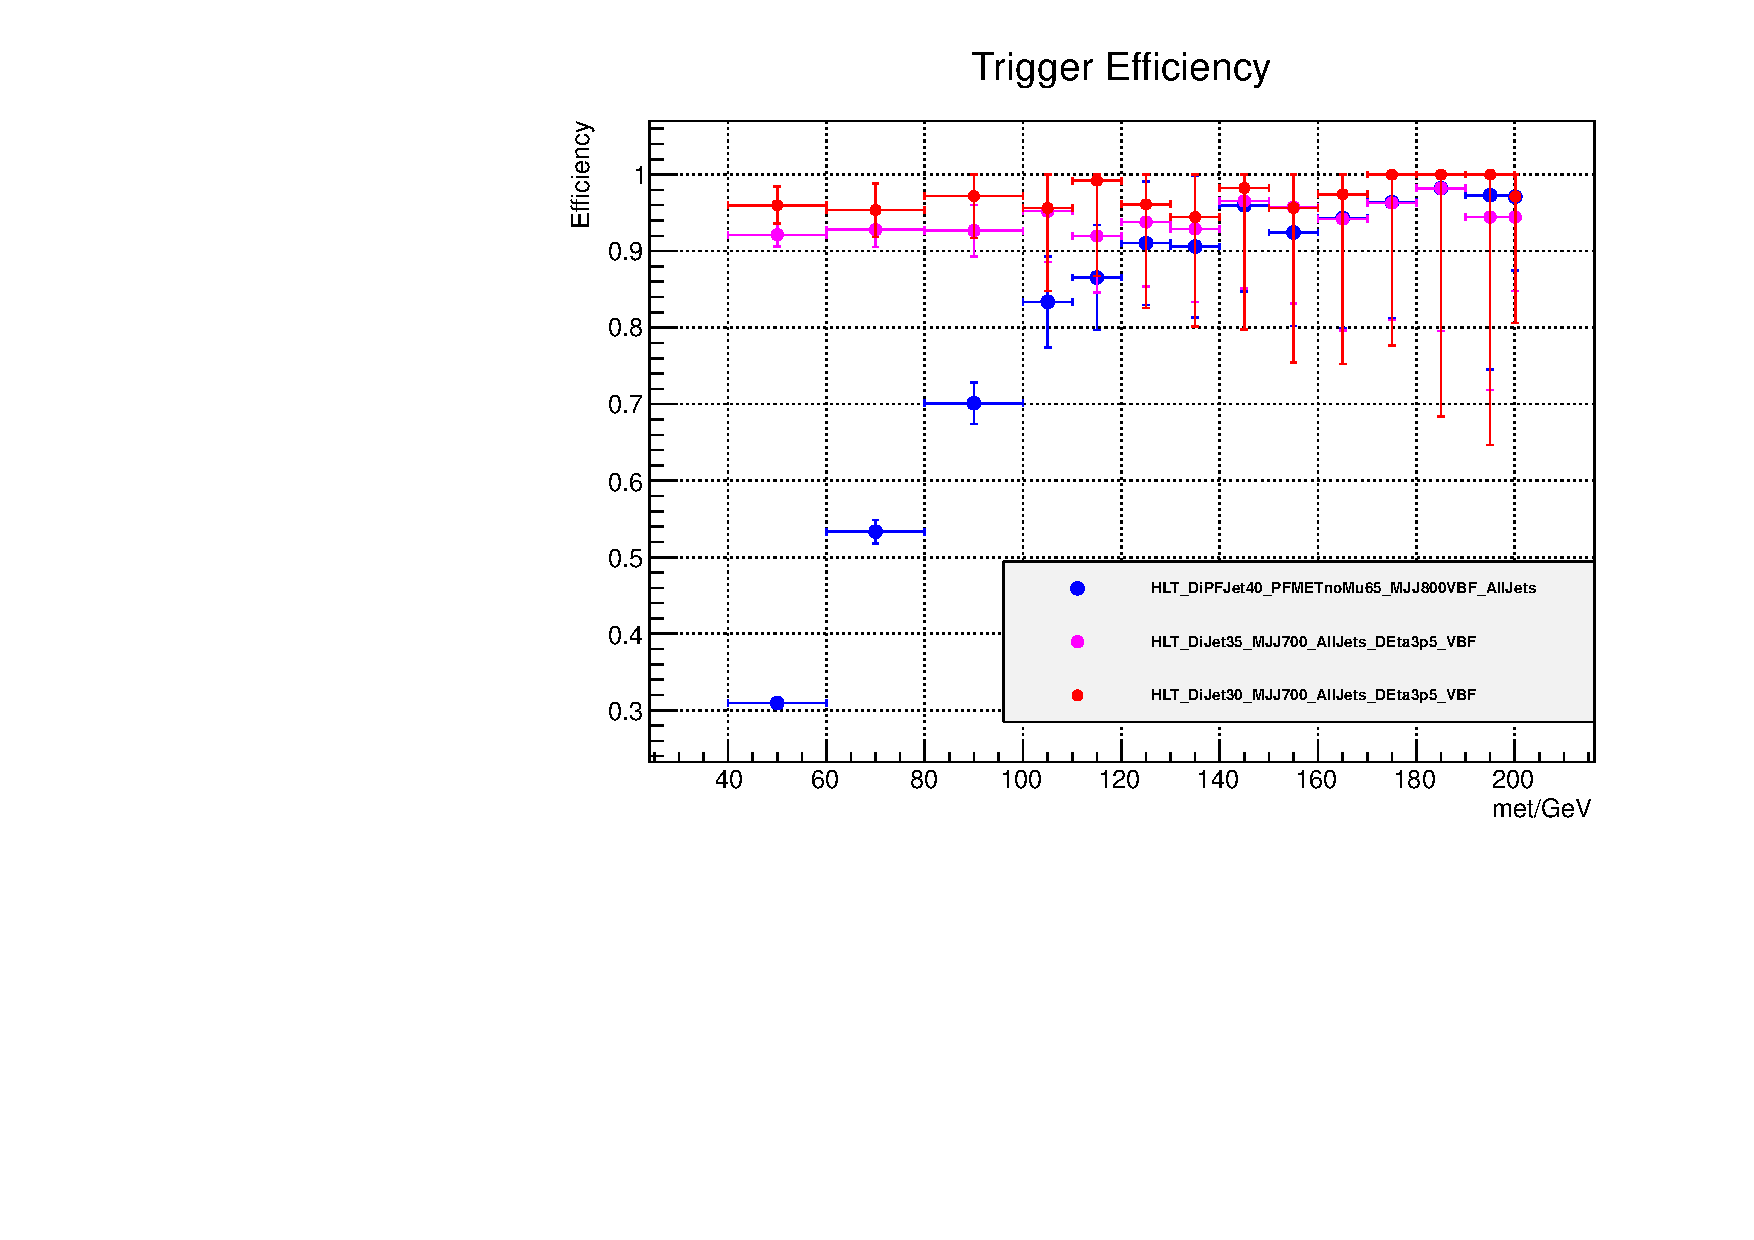
\includegraphics[width=\textwidth]{TalkPics/trigeffplots_hltonly/metefficiency.pdf}
    \end{block}
    \column{.55\textwidth}
    \begin{block}{\scriptsize No L1 cut}
      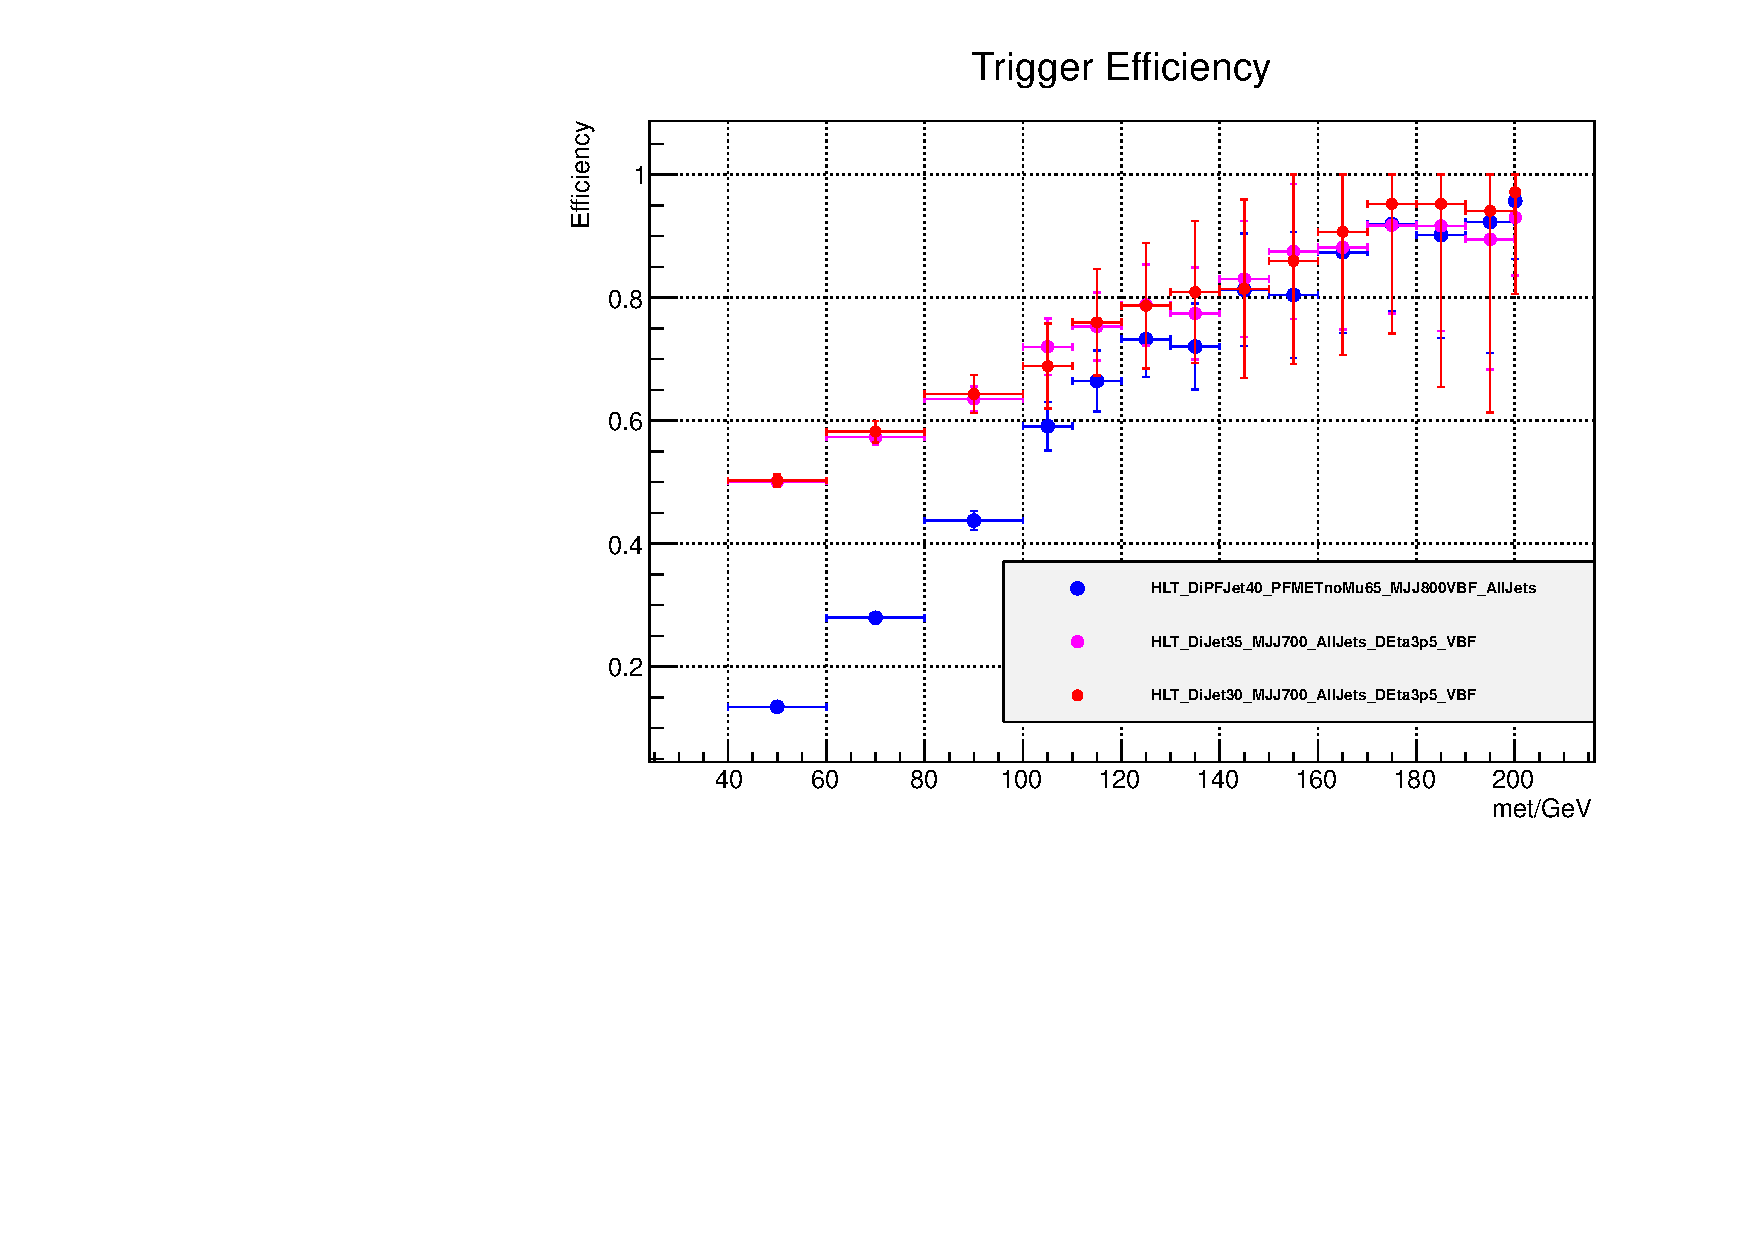
\includegraphics[width=\textwidth]{TalkPics/trigeffplots_nol1cut/metefficiency.pdf}
    \end{block}
  \end{columns}
\end{frame}

\begin{frame}
  \frametitle{$M_{jj}$}
  \begin{columns}
    \column{.55\textwidth}
    \begin{block}{\scriptsize L1 met $>$ 40 GeV}
      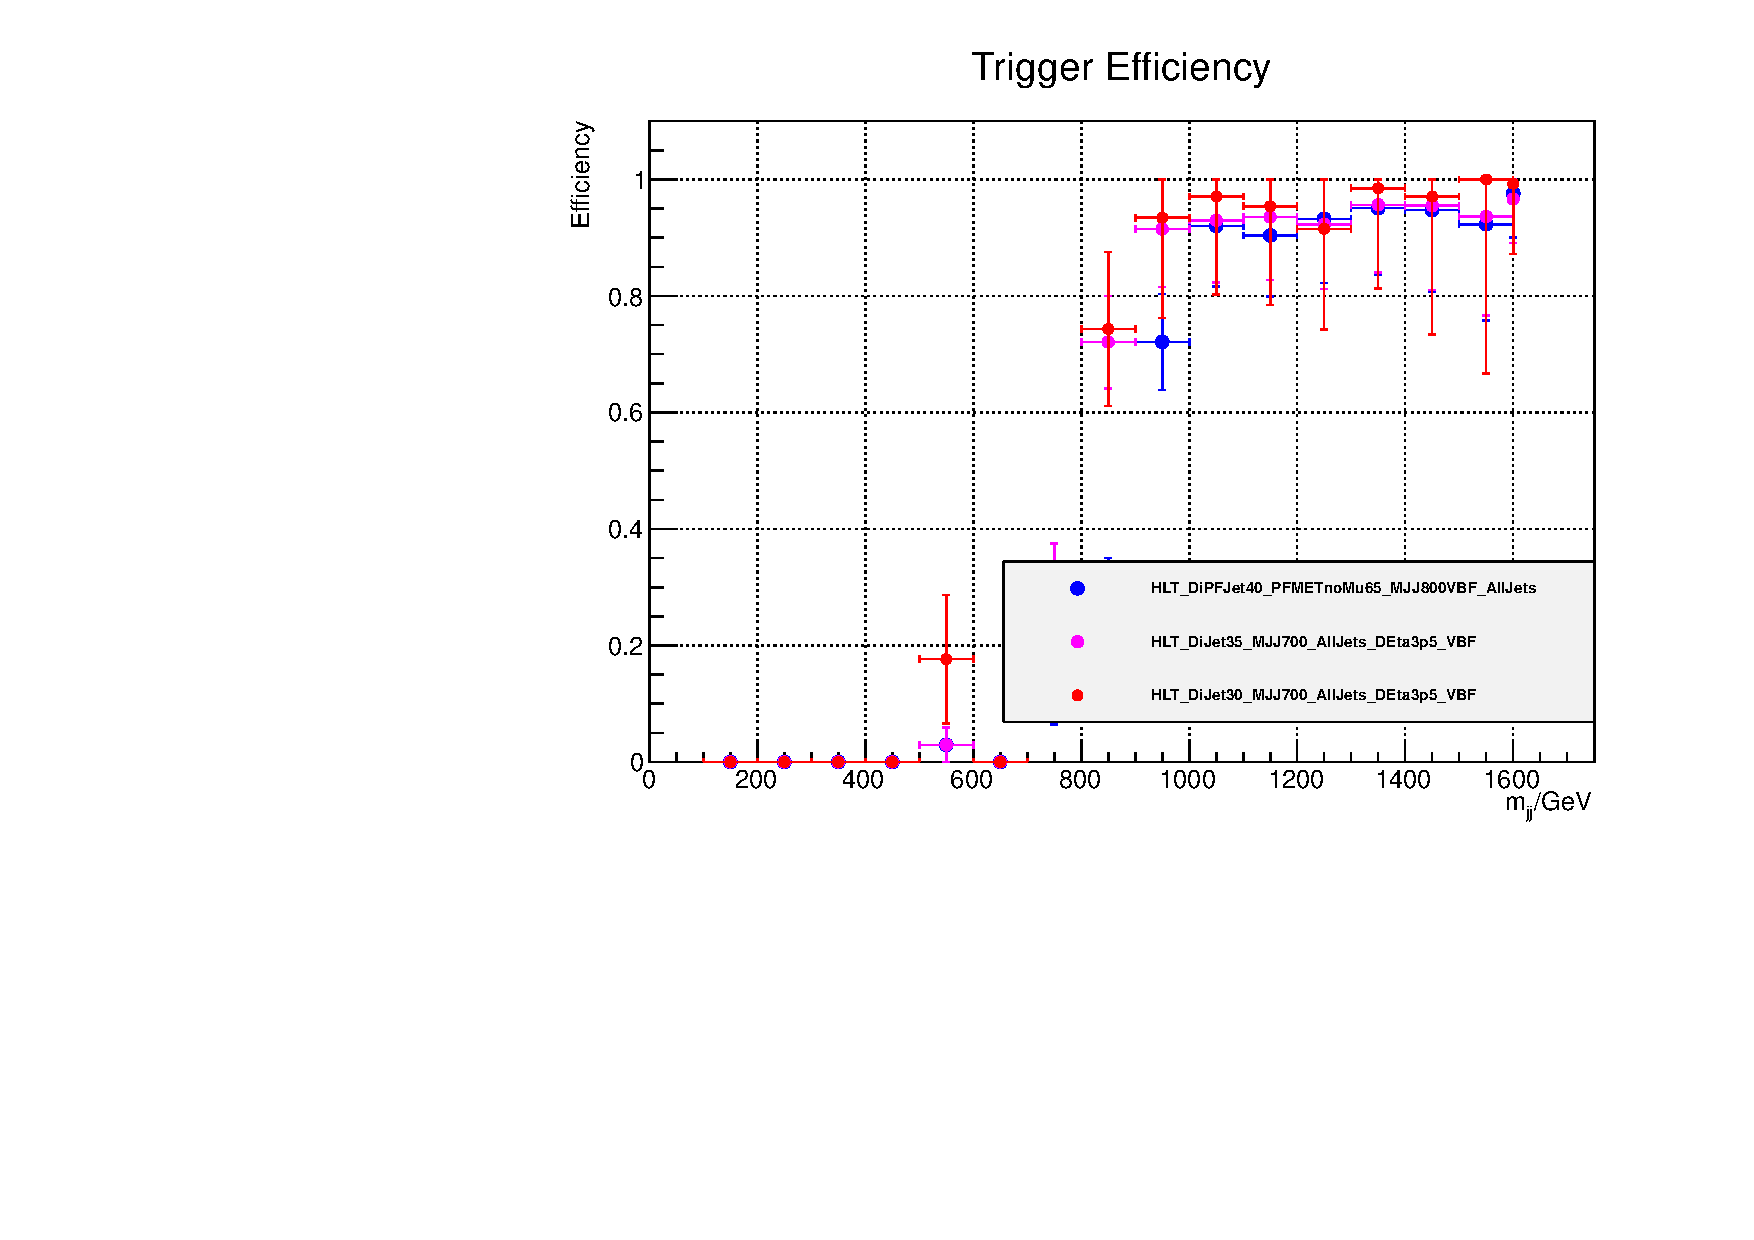
\includegraphics[width=\textwidth]{TalkPics/trigeffplots_hltonly/mjjefficiency.pdf}
    \end{block}
    \column{.55\textwidth}
    \begin{block}{\scriptsize No L1 cut}
      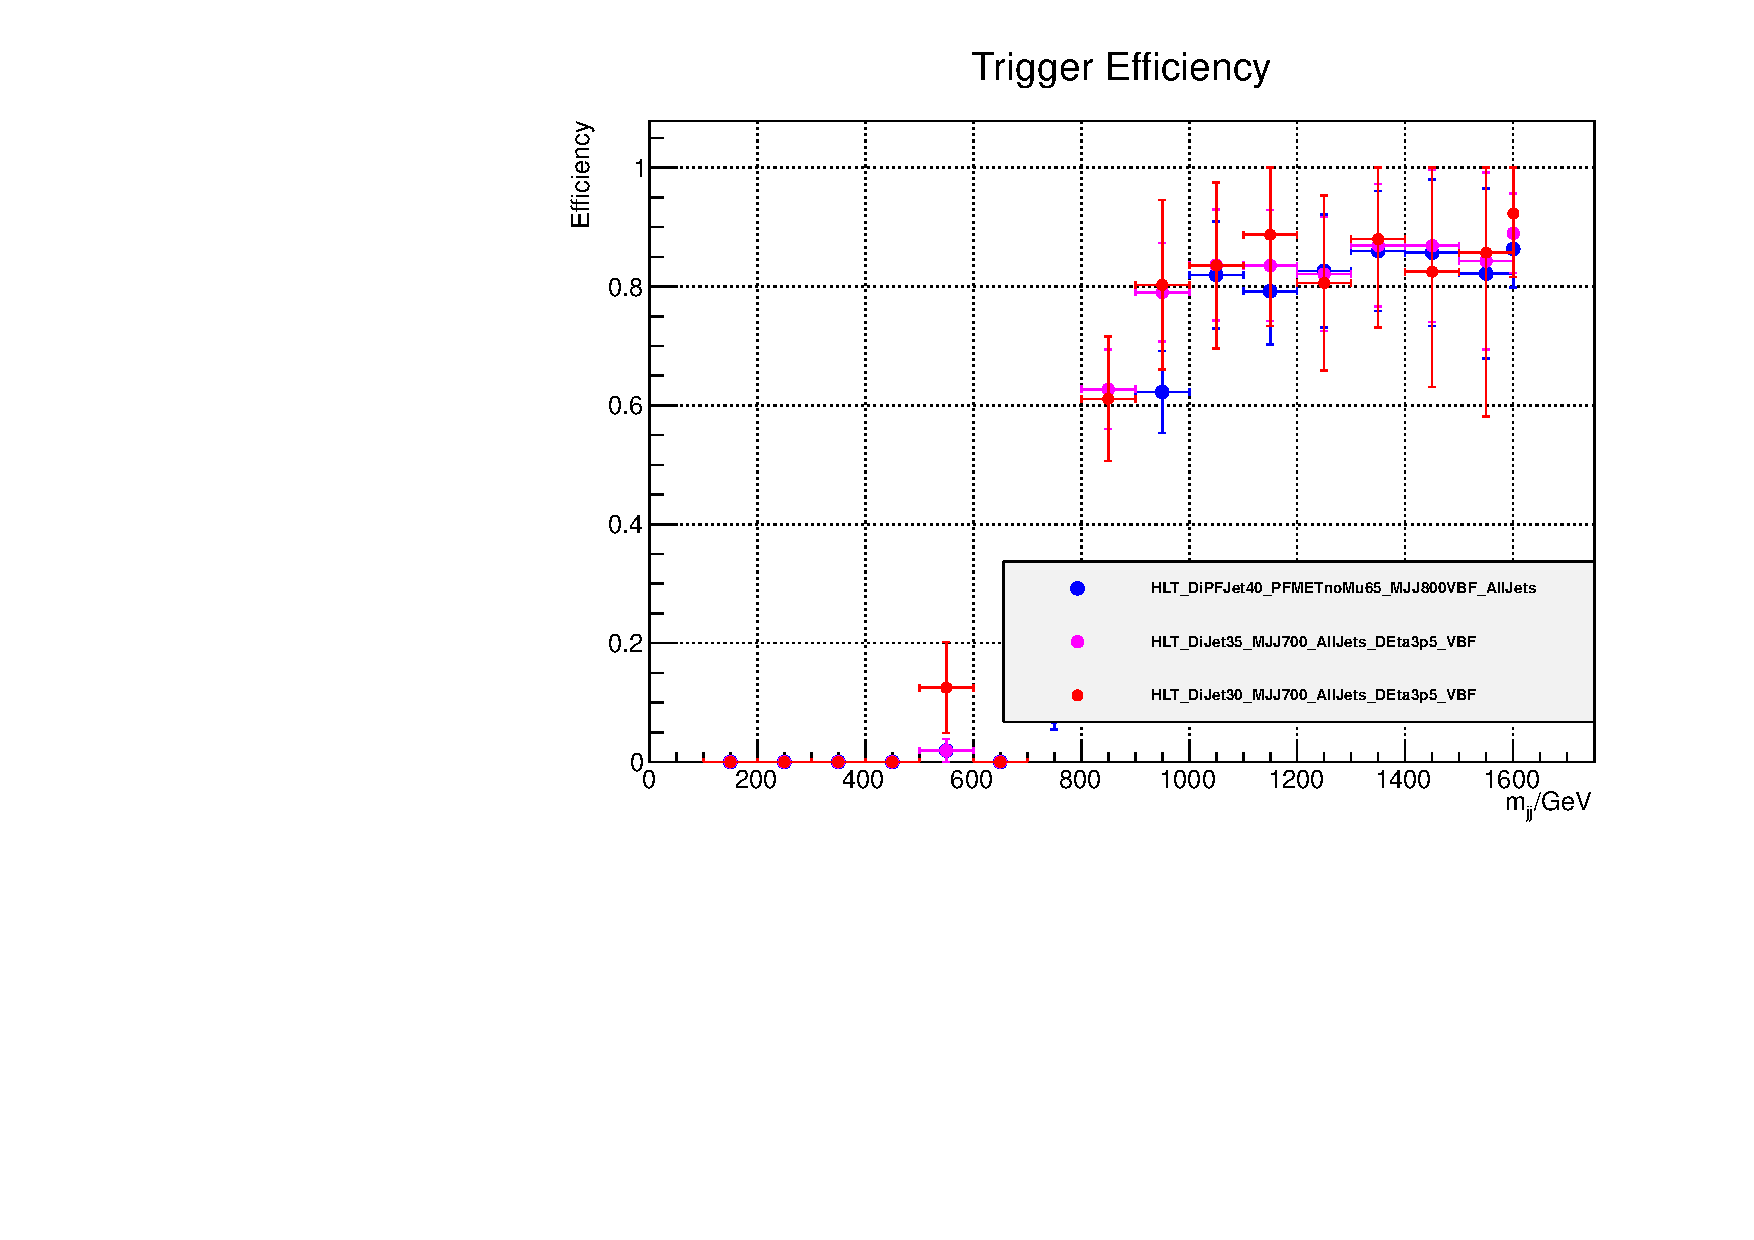
\includegraphics[width=\textwidth]{TalkPics/trigeffplots_nol1cut/mjjefficiency.pdf}
    \end{block}
  \end{columns}
\end{frame}

\begin{frame}
  \frametitle{Jet 2 pt}
  \begin{columns}
    \column{.55\textwidth}
    \begin{block}{\scriptsize L1 met $>$ 40 GeV}
      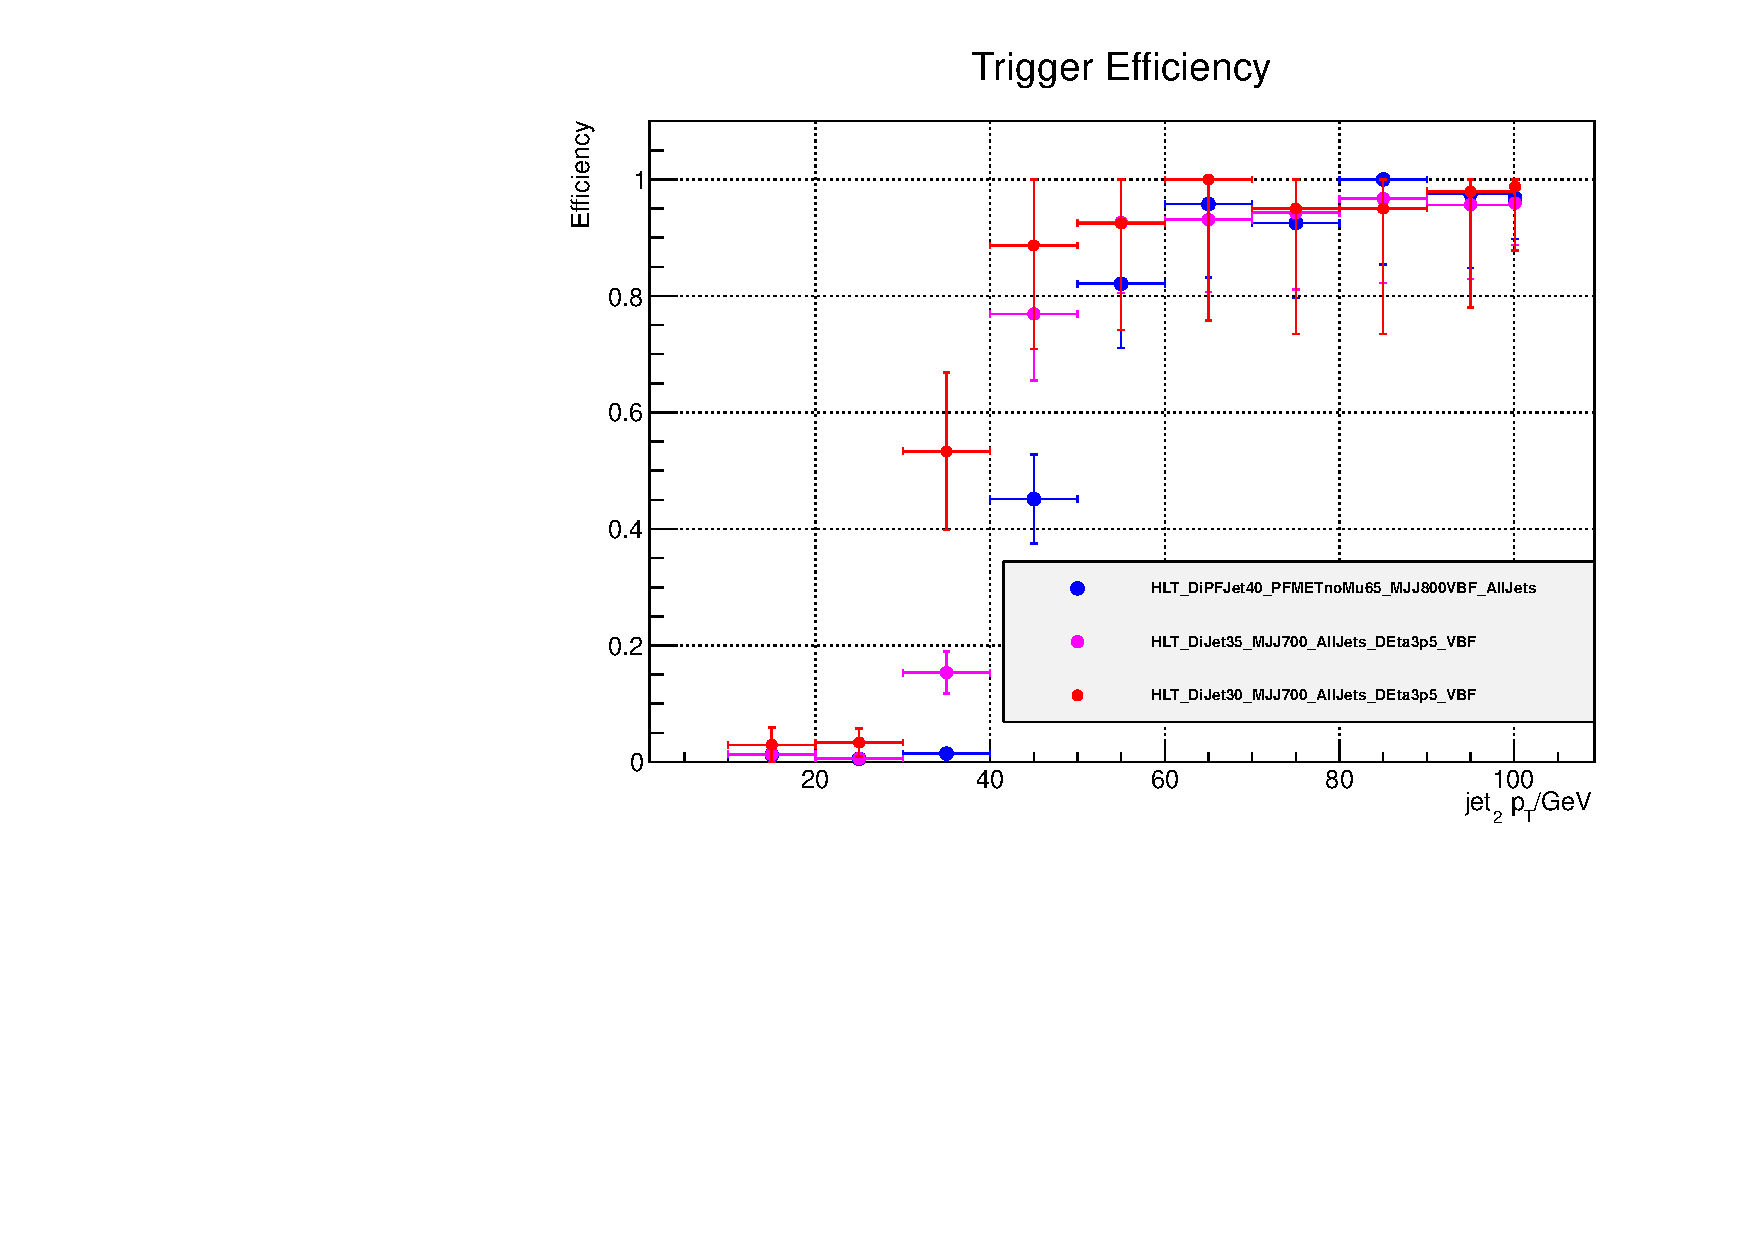
\includegraphics[width=\textwidth]{TalkPics/trigeffplots_hltonly/j2ptefficiency.pdf}
    \end{block}
    \column{.55\textwidth}
    \begin{block}{\scriptsize No L1 cut}
      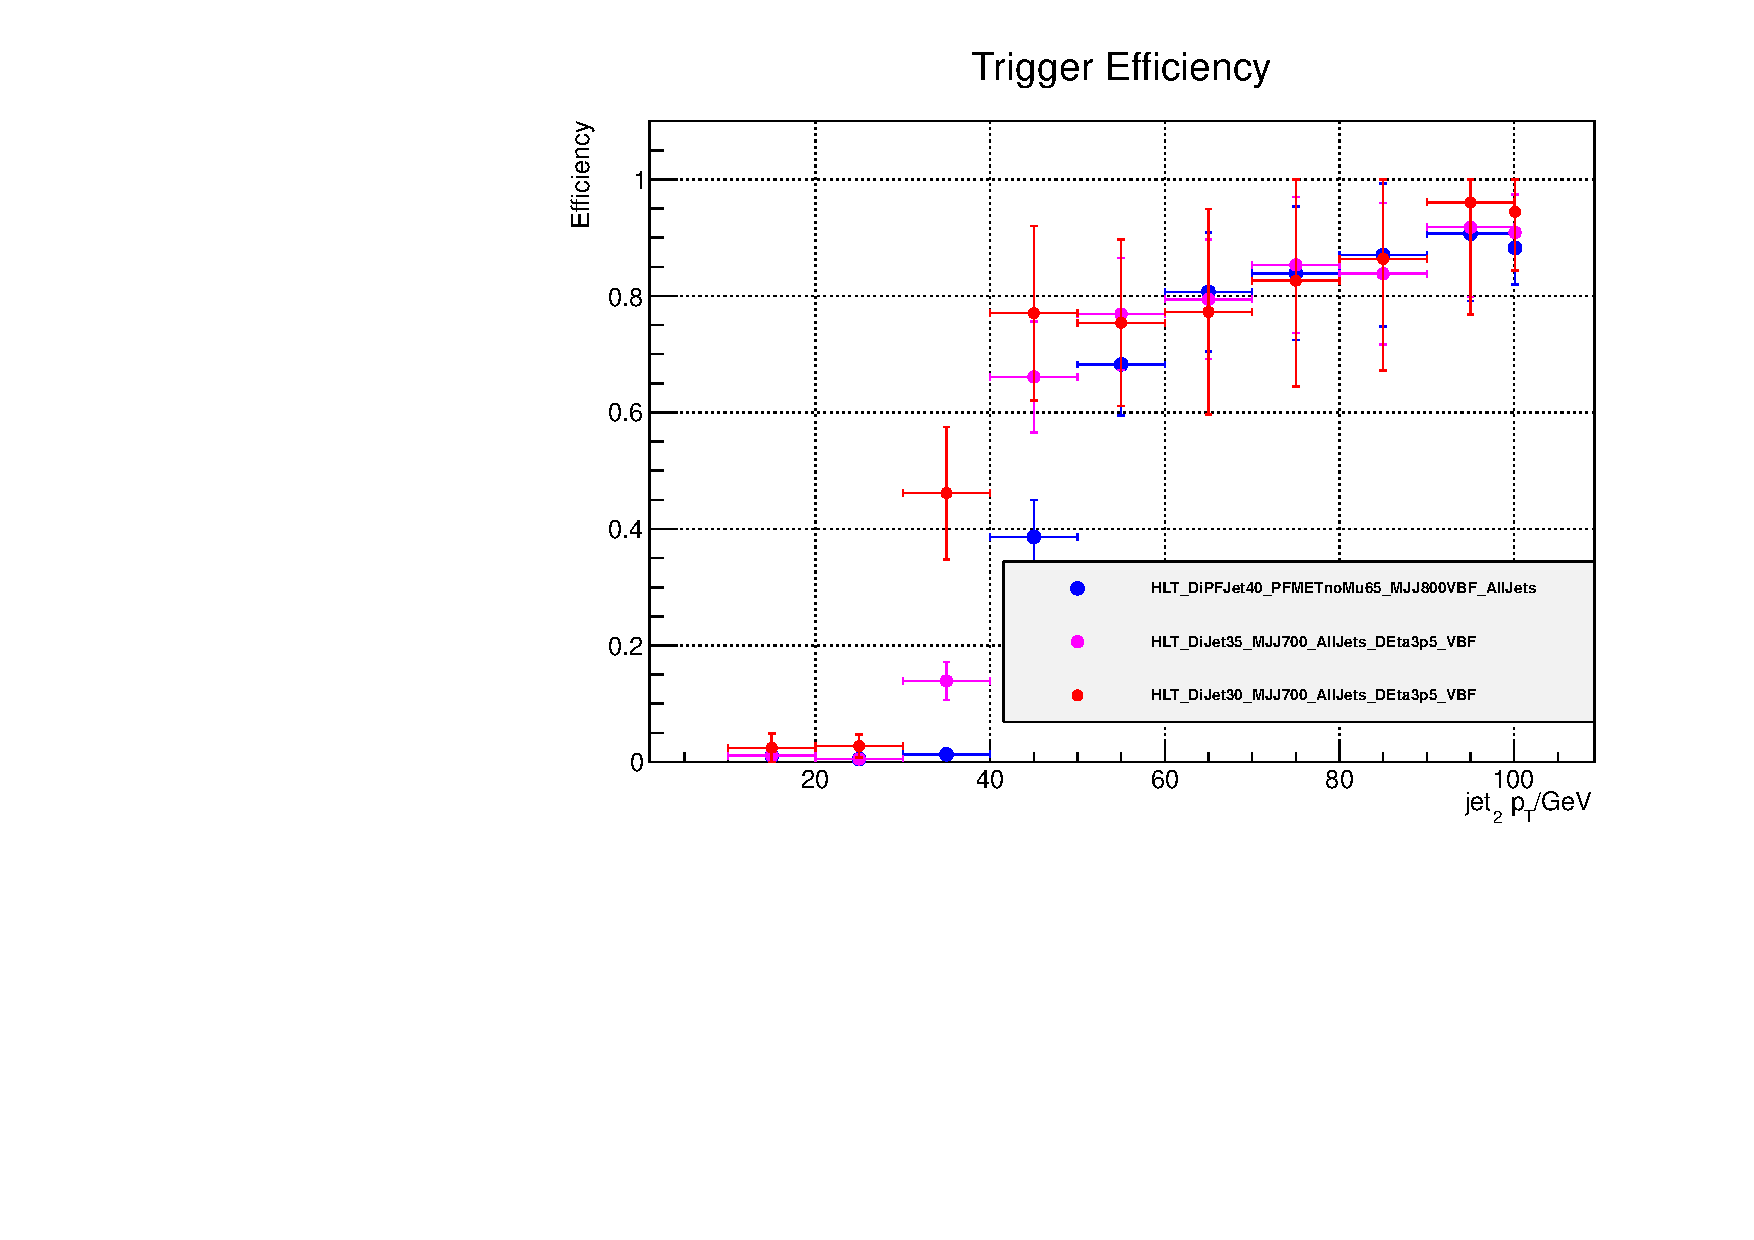
\includegraphics[width=\textwidth]{TalkPics/trigeffplots_nol1cut/j2ptefficiency.pdf}
    \end{block}
  \end{columns}
\end{frame}

\begin{frame}
  \frametitle{$\Delta\eta_{jj}$}
  \begin{columns}
    \column{.55\textwidth}
    \begin{block}{\scriptsize L1 met $>$ 40 GeV}
      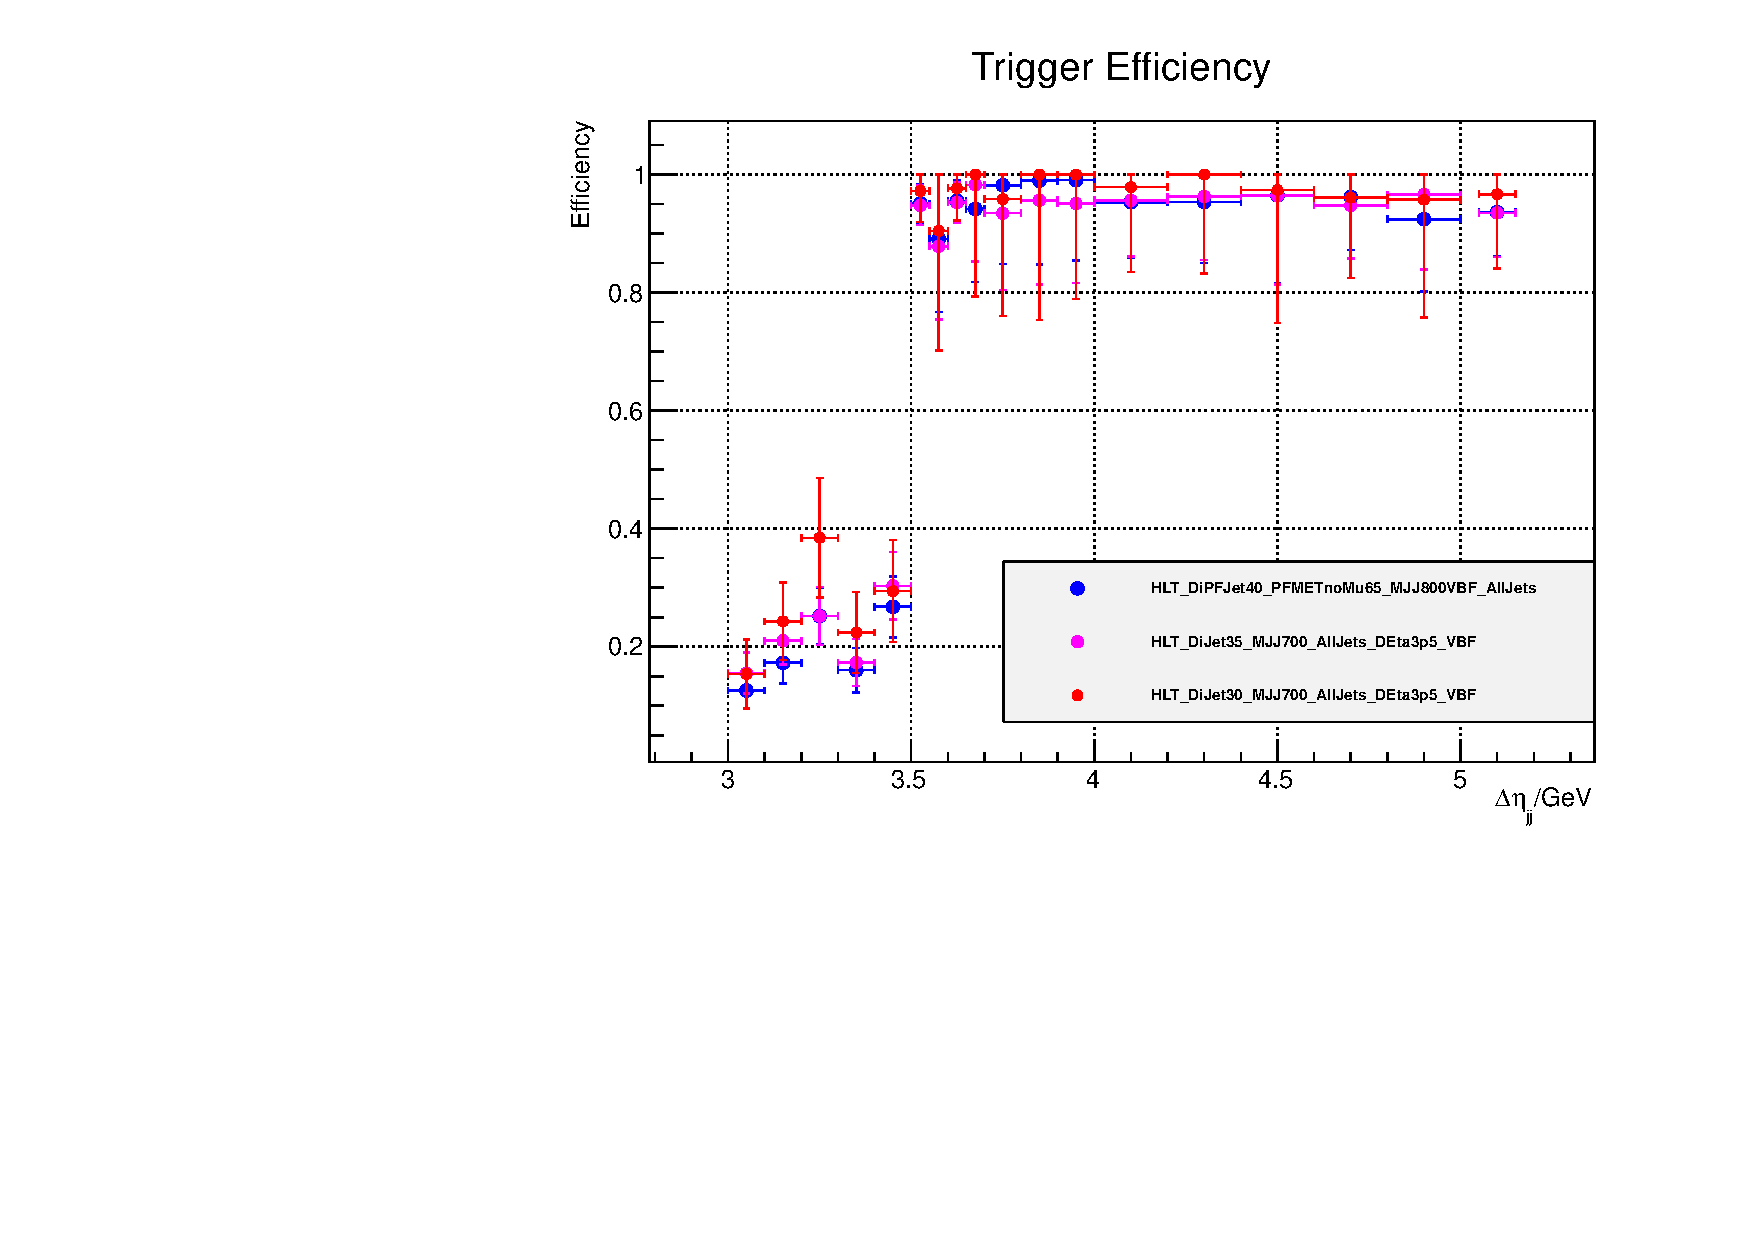
\includegraphics[width=\textwidth]{TalkPics/trigeffplots_hltonly/detaefficiency.pdf}
    \end{block}
    \column{.55\textwidth}
    \begin{block}{\scriptsize No L1 cut}
      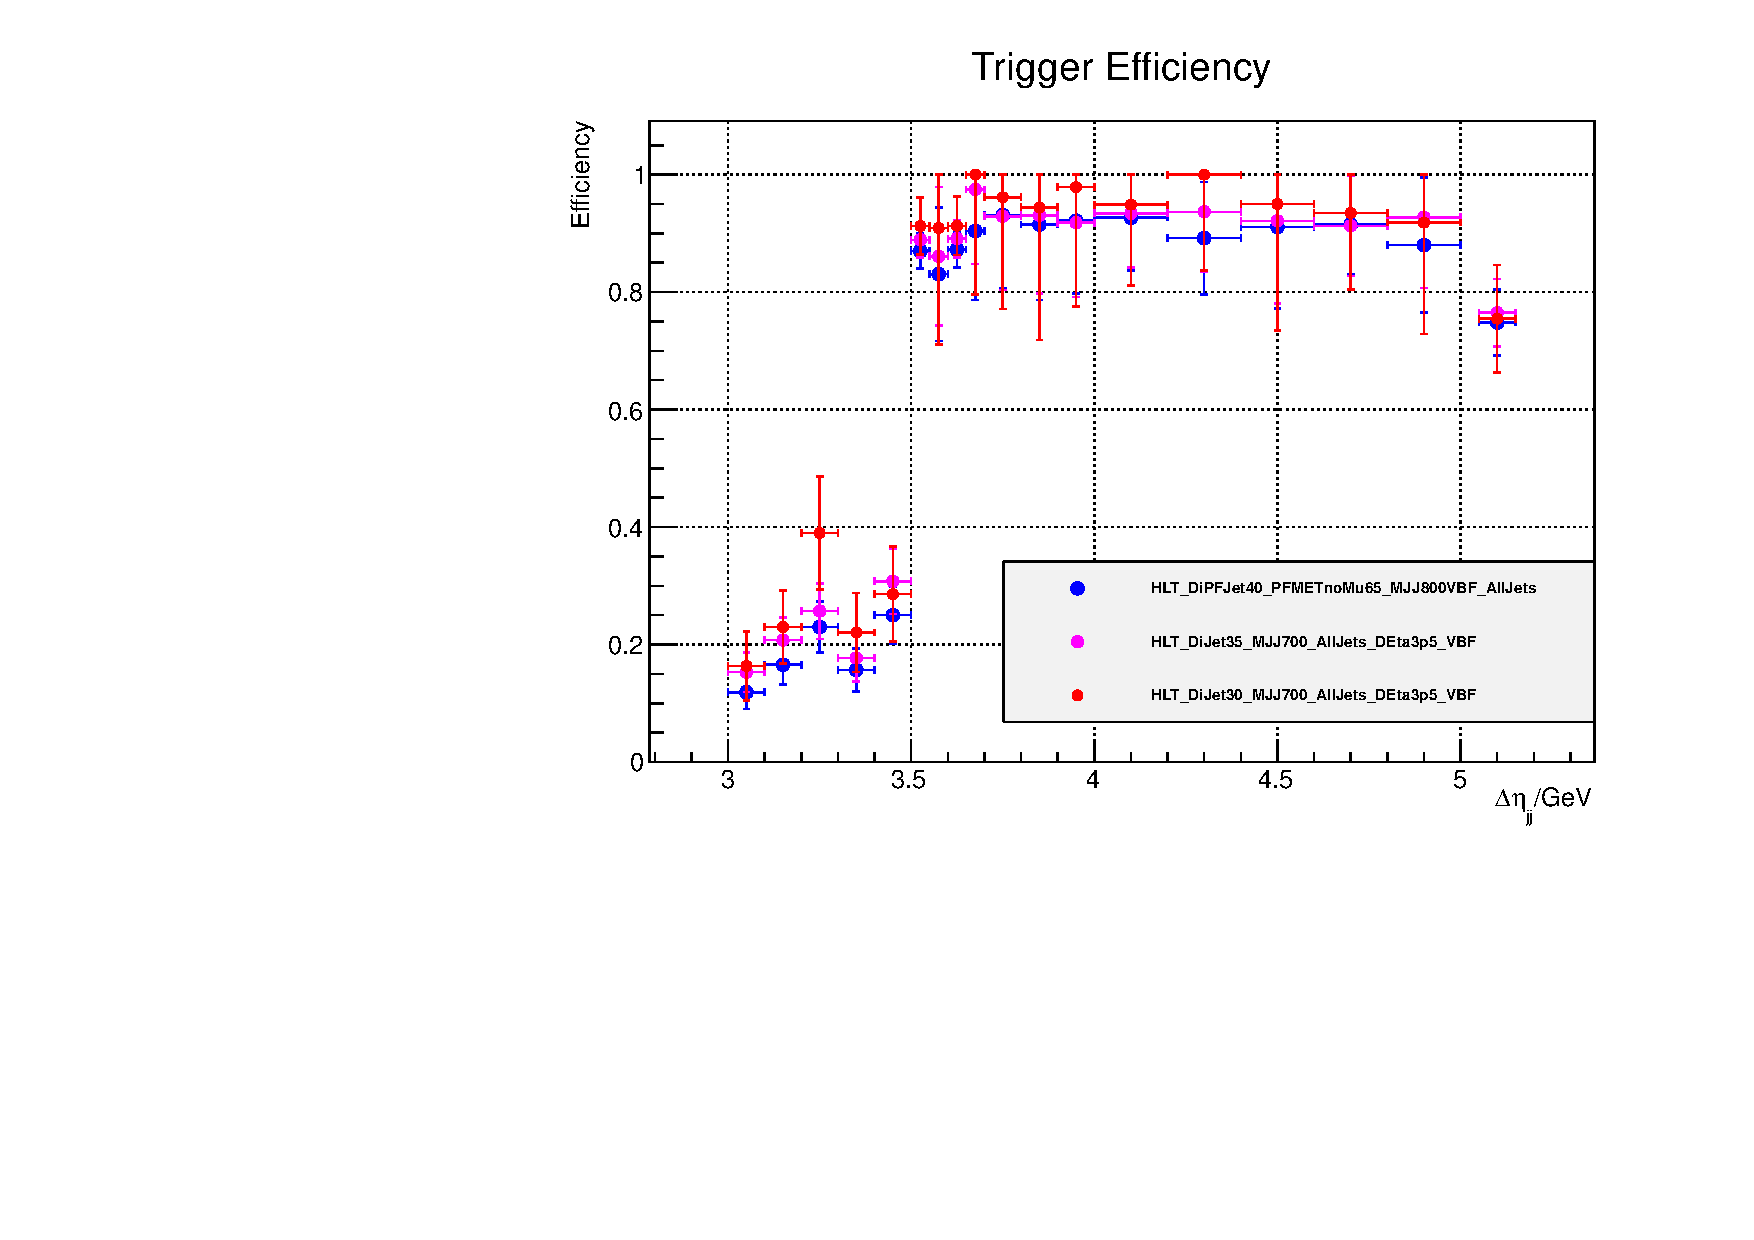
\includegraphics[width=\textwidth]{TalkPics/trigeffplots_nol1cut/detaefficiency.pdf}
    \end{block}
  \end{columns}
\end{frame}

\begin{frame}
  \frametitle{3D Efficiencies}
  \begin{block}{}
    \begin{itemize}
    \item Picked bins in mjj, met and jet 2 pt cut
    \item Statistics are very limited when more than about 3 bins are used for each variable
    \item[-] jet 1 pt cut was relaxed to 30 GeV to increase stats
    \end{itemize}
  \end{block}
\end{frame}

\begin{frame}
  \vspace{-.4cm}
    \begin{block}{HLT\_DiJet35, $120<met<160$}
      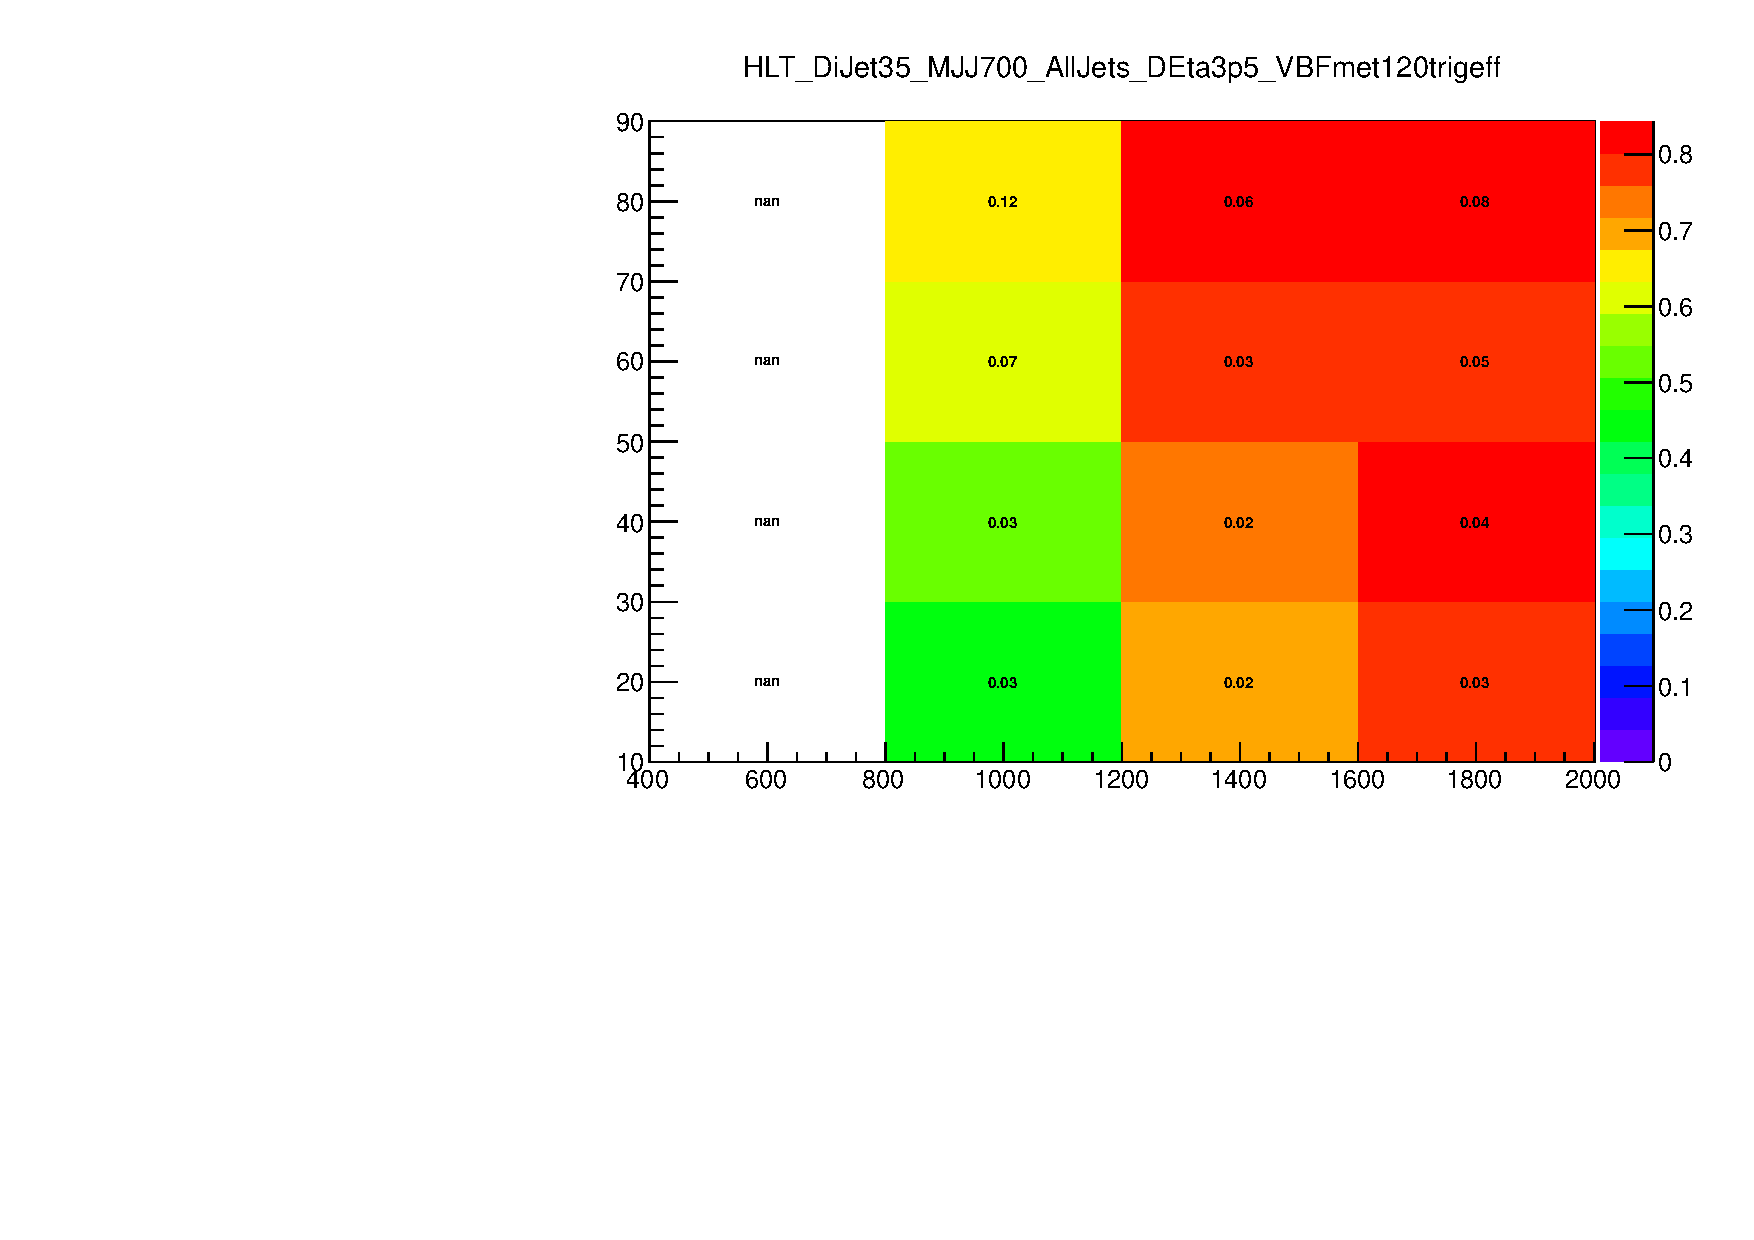
\includegraphics[clip=true,trim=0 10 0 20,width=\textwidth]{TalkPics/HLT_DiJet35_MJJ700_AllJets_DEta3p5_VBFmet120trigeff.pdf}
    \end{block}
\end{frame}

\begin{frame}
  \vspace{-.4cm}
    \begin{block}{HLT\_DiJet30, $120<met<160$}
      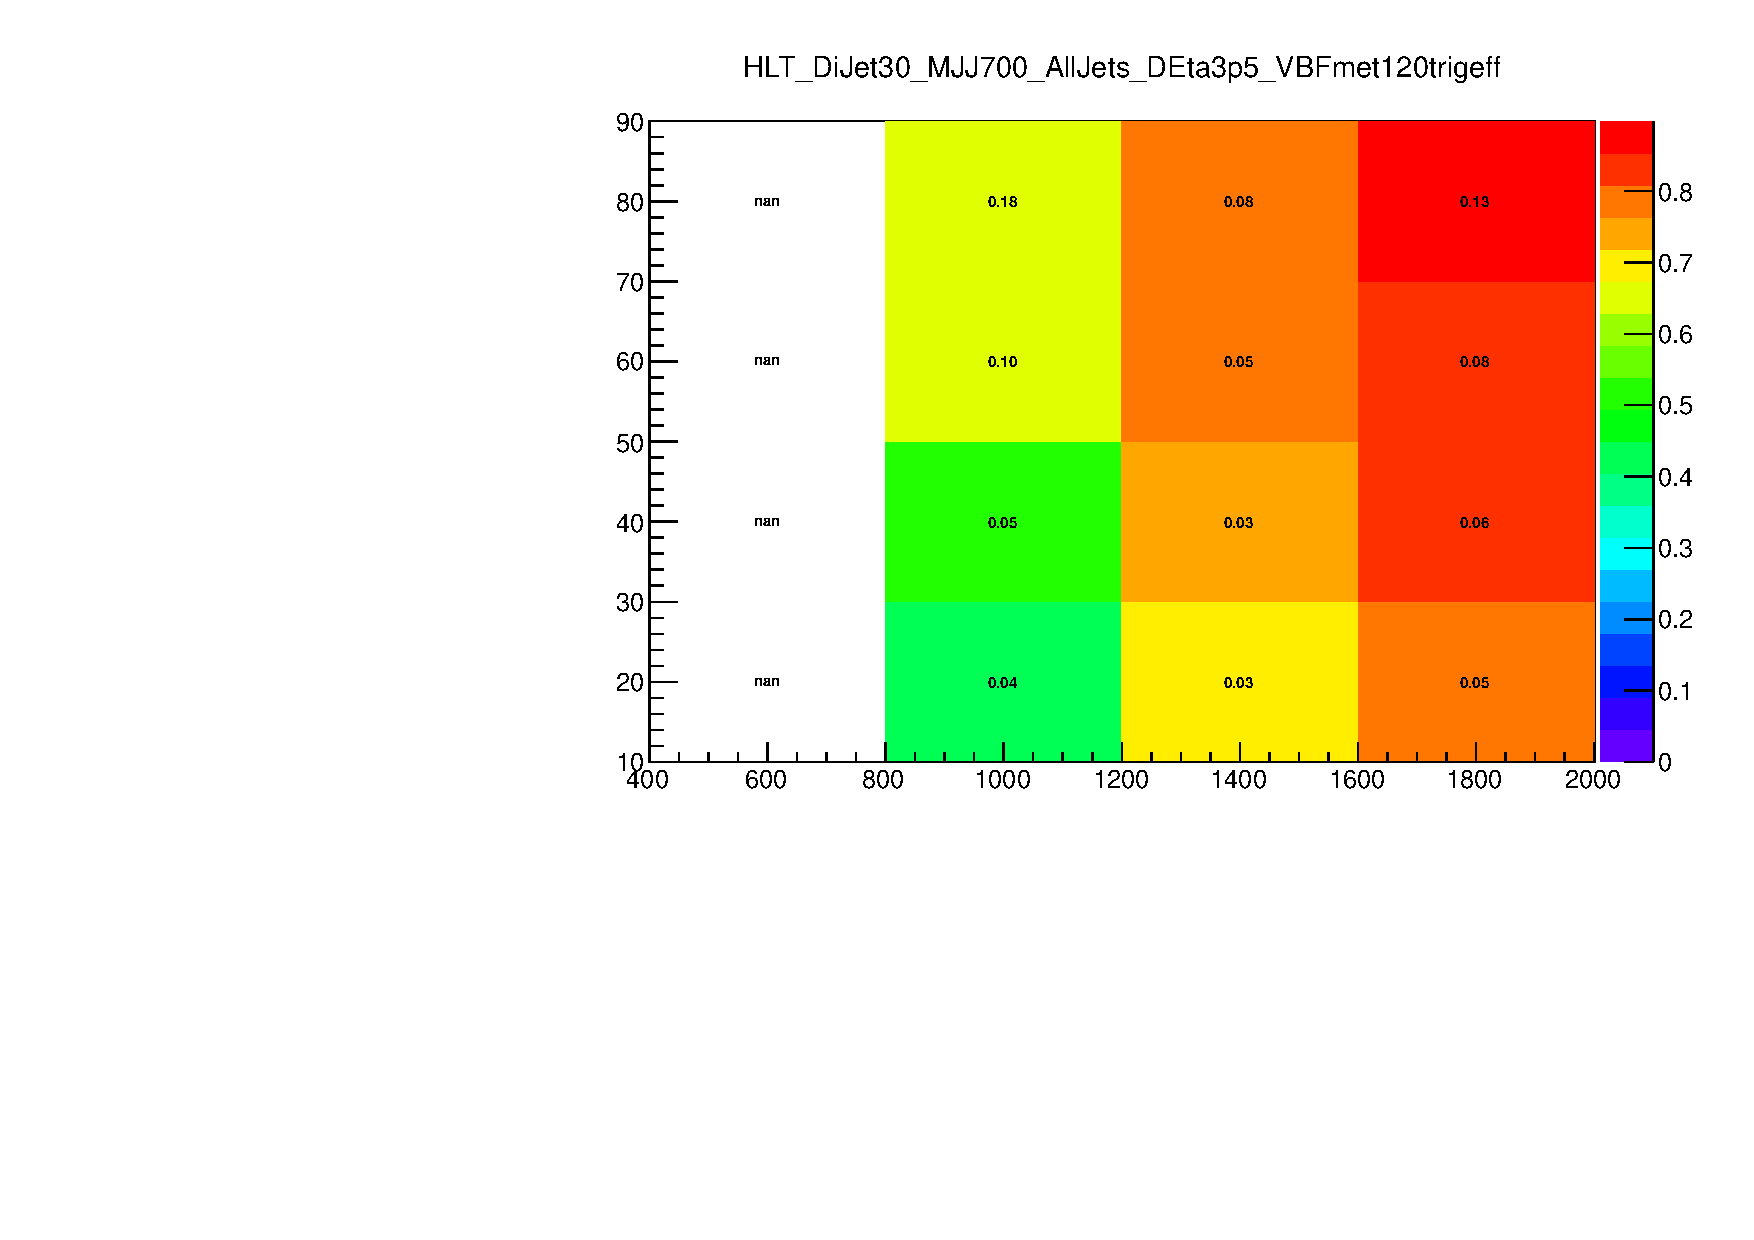
\includegraphics[clip=true,trim=0 10 0 20,width=\textwidth]{TalkPics/HLT_DiJet30_MJJ700_AllJets_DEta3p5_VBFmet120trigeff.pdf}
    \end{block}
\end{frame}

\begin{frame}
  \frametitle{Conclusions}
  \label{lastframe}

  \begin{block}{}
    \scriptsize
    \begin{itemize}
    \item Shape differences seen before between my and Phat's curves seem to be due to L1 met cut
    \item $\Delta\eta_{jj}$ turn on curve seems very sharp
    \item[-] We therefore have the option of relaxing our offline cut or increasing the trigger threshold in future
    \end{itemize}
  \end{block}

  \begin{block}{}
    \scriptsize
    \begin{itemize}
    \item 3D trigger efficiency work is in progress
    \item Code to write 1D efficiencies into format read in by analysis frameworks is being written
    \end{itemize}
  \end{block}

\end{frame}

\begin{frame}
  \frametitle{Backup}
\end{frame}

\begin{frame}
  \frametitle{Phat's efficiencies - met}
  \centering
  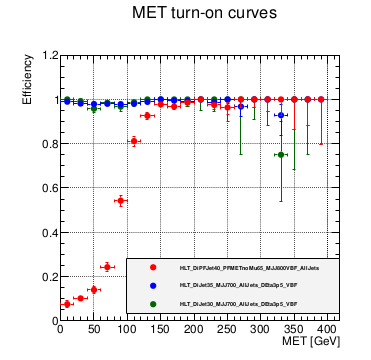
\includegraphics[width=.5\textwidth]{TalkPics/phattrigeffmet.png}
\end{frame}

\begin{frame}
  \frametitle{Phat's efficiencies - mjj}
  \centering
  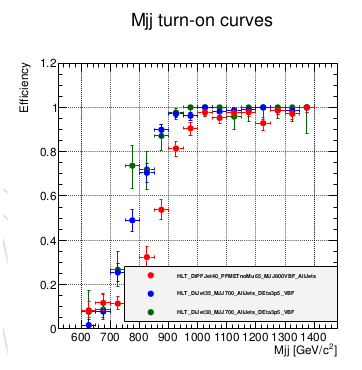
\includegraphics[width=.5\textwidth]{TalkPics/phattrigeffmjj.png}
\end{frame}

\begin{frame}
  \frametitle{Phat's efficiencies - j2pt}
  \centering
  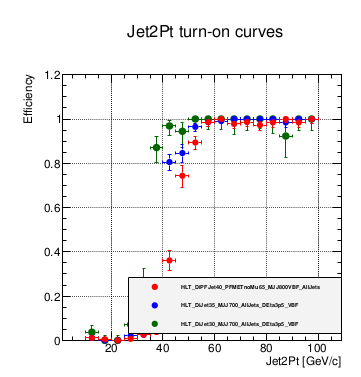
\includegraphics[width=.5\textwidth]{TalkPics/phattrigeffj2pt.png}
\end{frame}

\begin{frame}
  \frametitle{Phat's efficiencies - l1met}
  \centering
  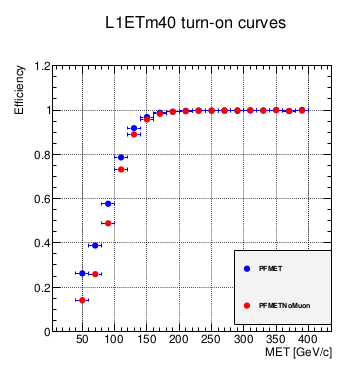
\includegraphics[width=.5\textwidth]{TalkPics/phattrigeffl1met.png}
\end{frame}

\end{fmffile}
\end{document}
